\chapter{Application}
\label{ch:application}

The application is a local web app in the style of a team chat client: a channel on the left and a tasks panel on the right with \emph{Needs you} (suggestions the current person may decide), the person's or the team's tasks, and \emph{Waiting on teammates}. Further pages show the dependency graph, a timeline and saved model results; every message has a ``How AI read this'' inspector. Messages are typed in \emph{Live AI} mode or replayed from scripted demo stories, whose extraction is pre-written but whose reconciliation, review and graph are the real code. A suggestion can be accepted, edited then accepted (edited fields are recorded as \emph{human}), dismissed, or, for a task nobody was named for, taken or left open for a volunteer. All screenshots were captured automatically from the app running the real checkpoints on 17 November 2026.


\begin{figure}[htbp]
\centering
\shot{01_workspace_needs_you}
\caption{The 17-message demo story viewed as Riya: the suggestions from her latest message wait for Bianca, the person they affect; Riya may only dismiss them or switch view.}
\label{fig:shotdemo}
\end{figure}

\begin{figure}[htbp]
\centering
\shot{06_live_extraction}
\caption{Live mode, viewed as Bianca: a named request with owner, due date and a deadline/schedule question; an unowned team request offering \emph{I'll take it} or \emph{Leave open}; and two non-actionable messages that produced no task.}
\label{fig:shotlive}
\end{figure}

\begin{figure}[htbp]
\centering
\begin{subfigure}[t]{0.49\linewidth}\centering
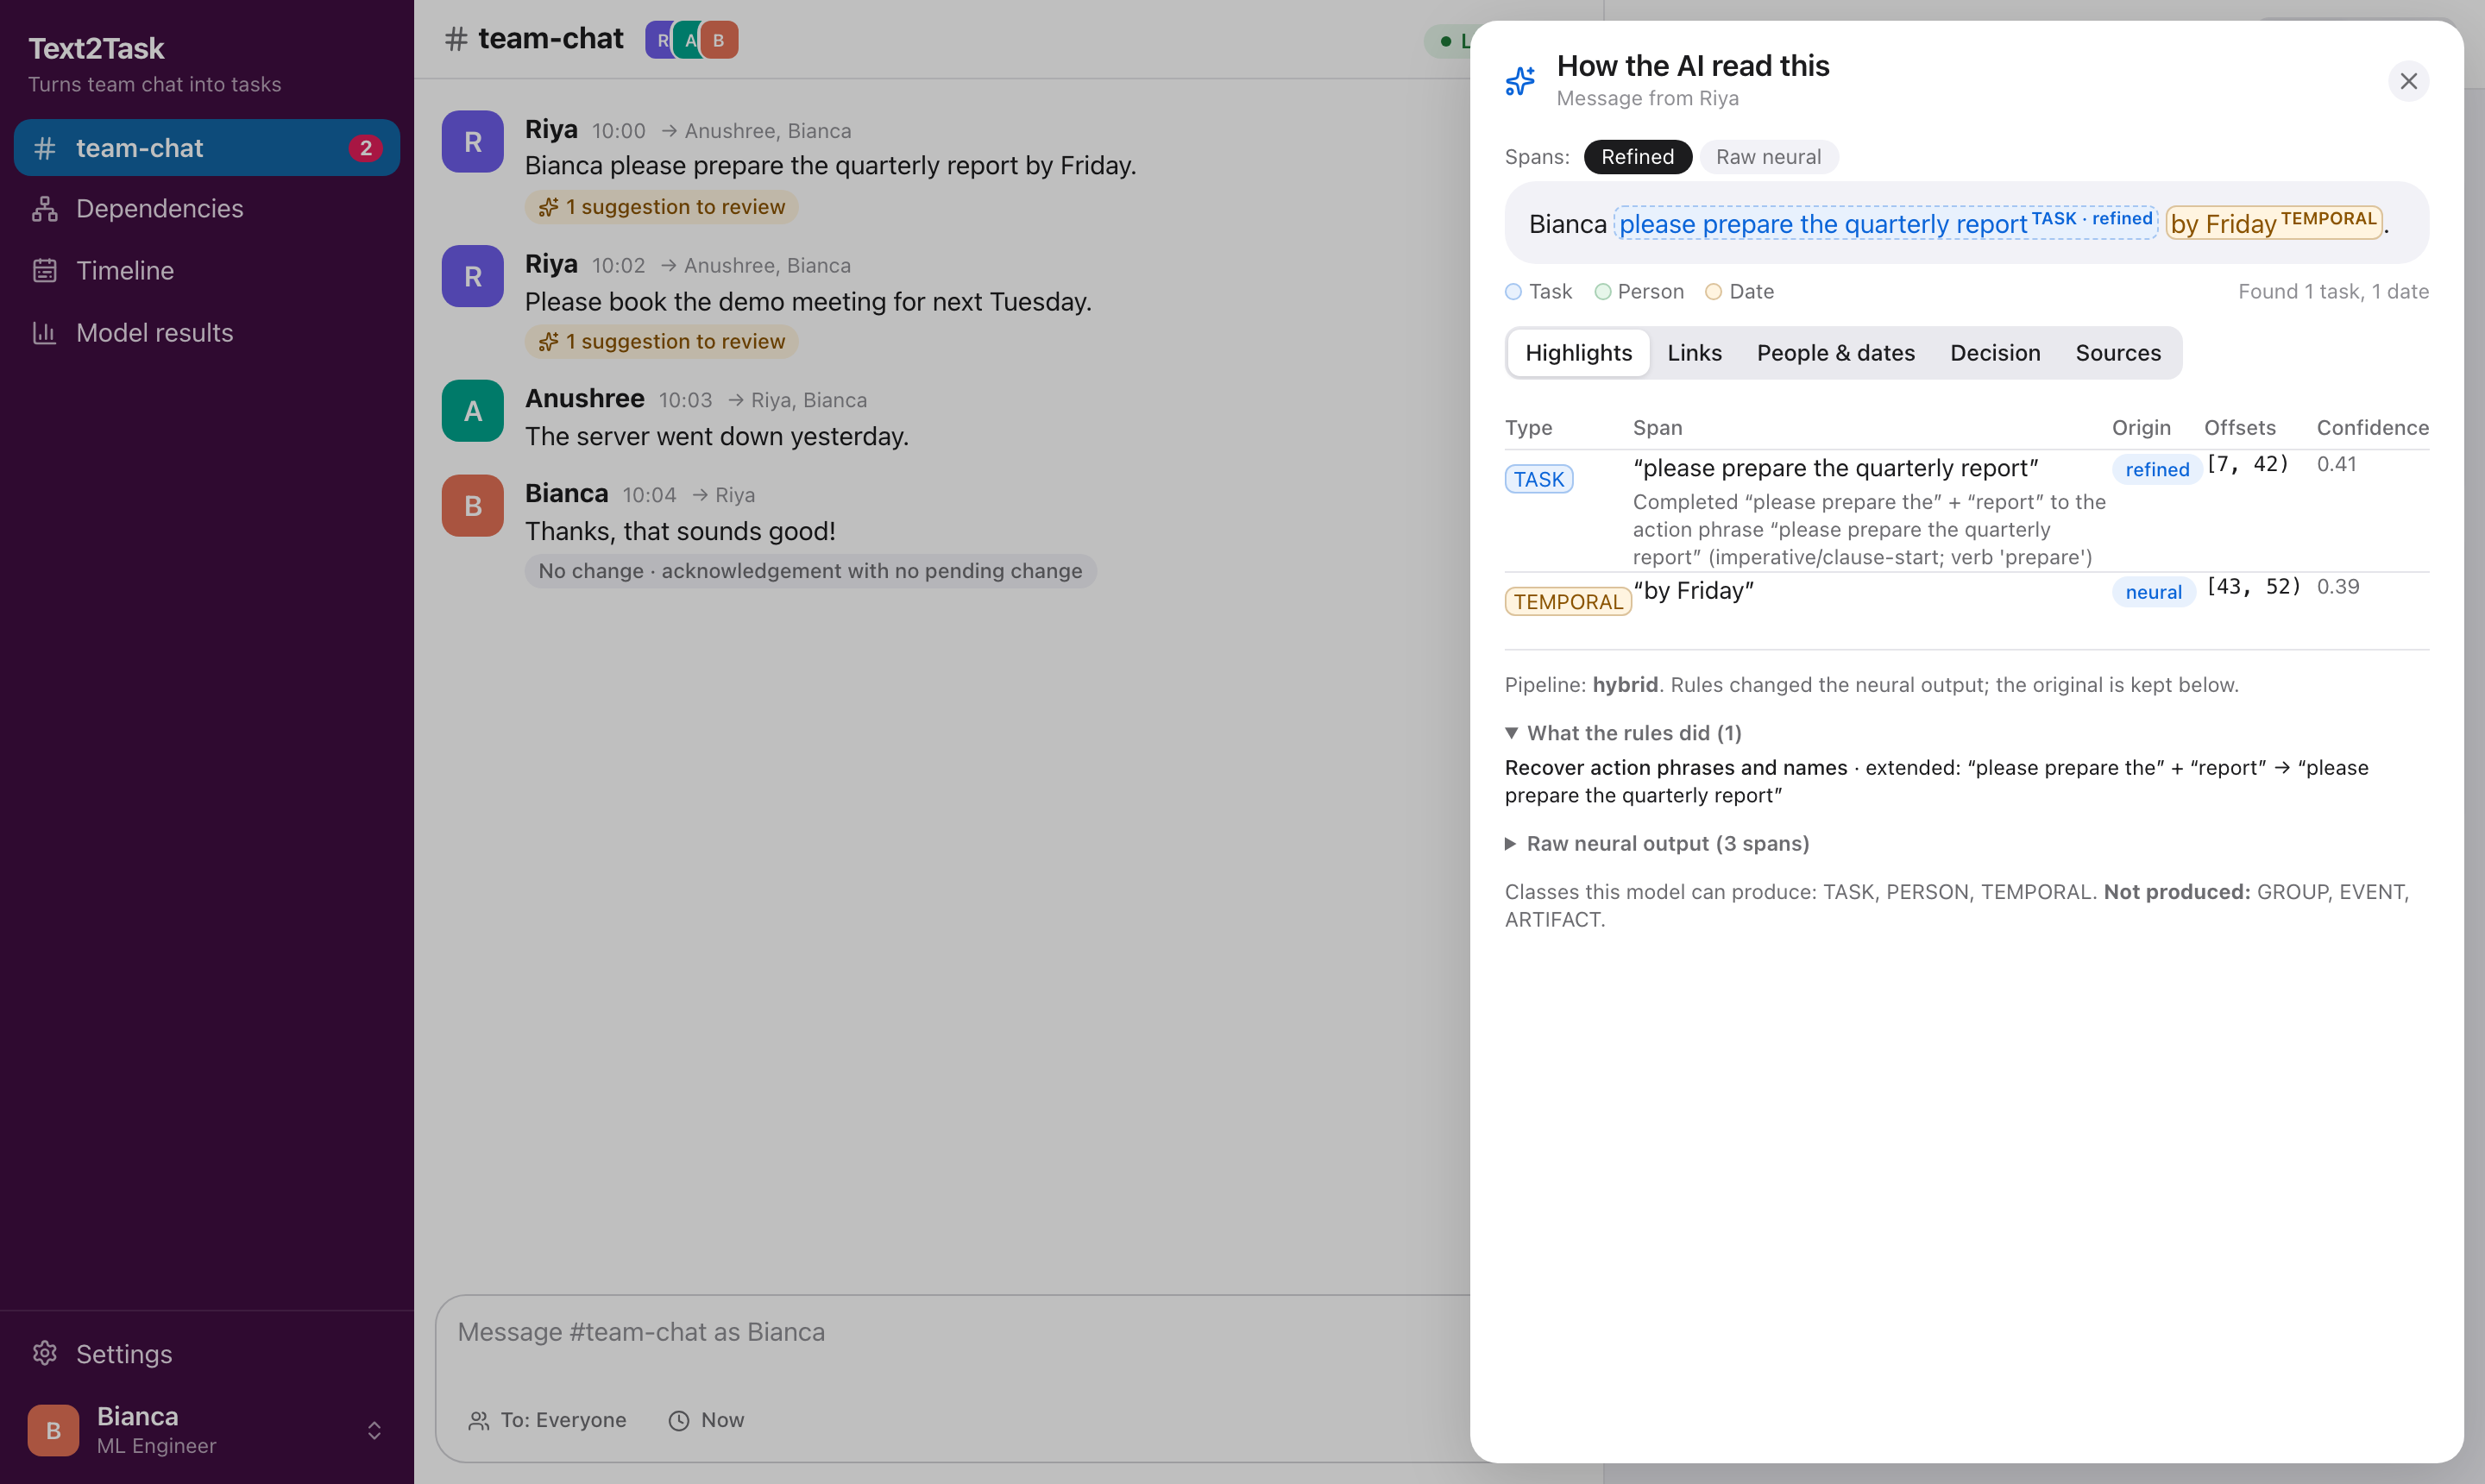
\includegraphics[width=\linewidth, trim=1690 520 20 0, clip]{figures/screenshots/07_inspector_hybrid.png}
\caption{Refined spans (hybrid)}\end{subfigure}\hfill
\begin{subfigure}[t]{0.49\linewidth}\centering
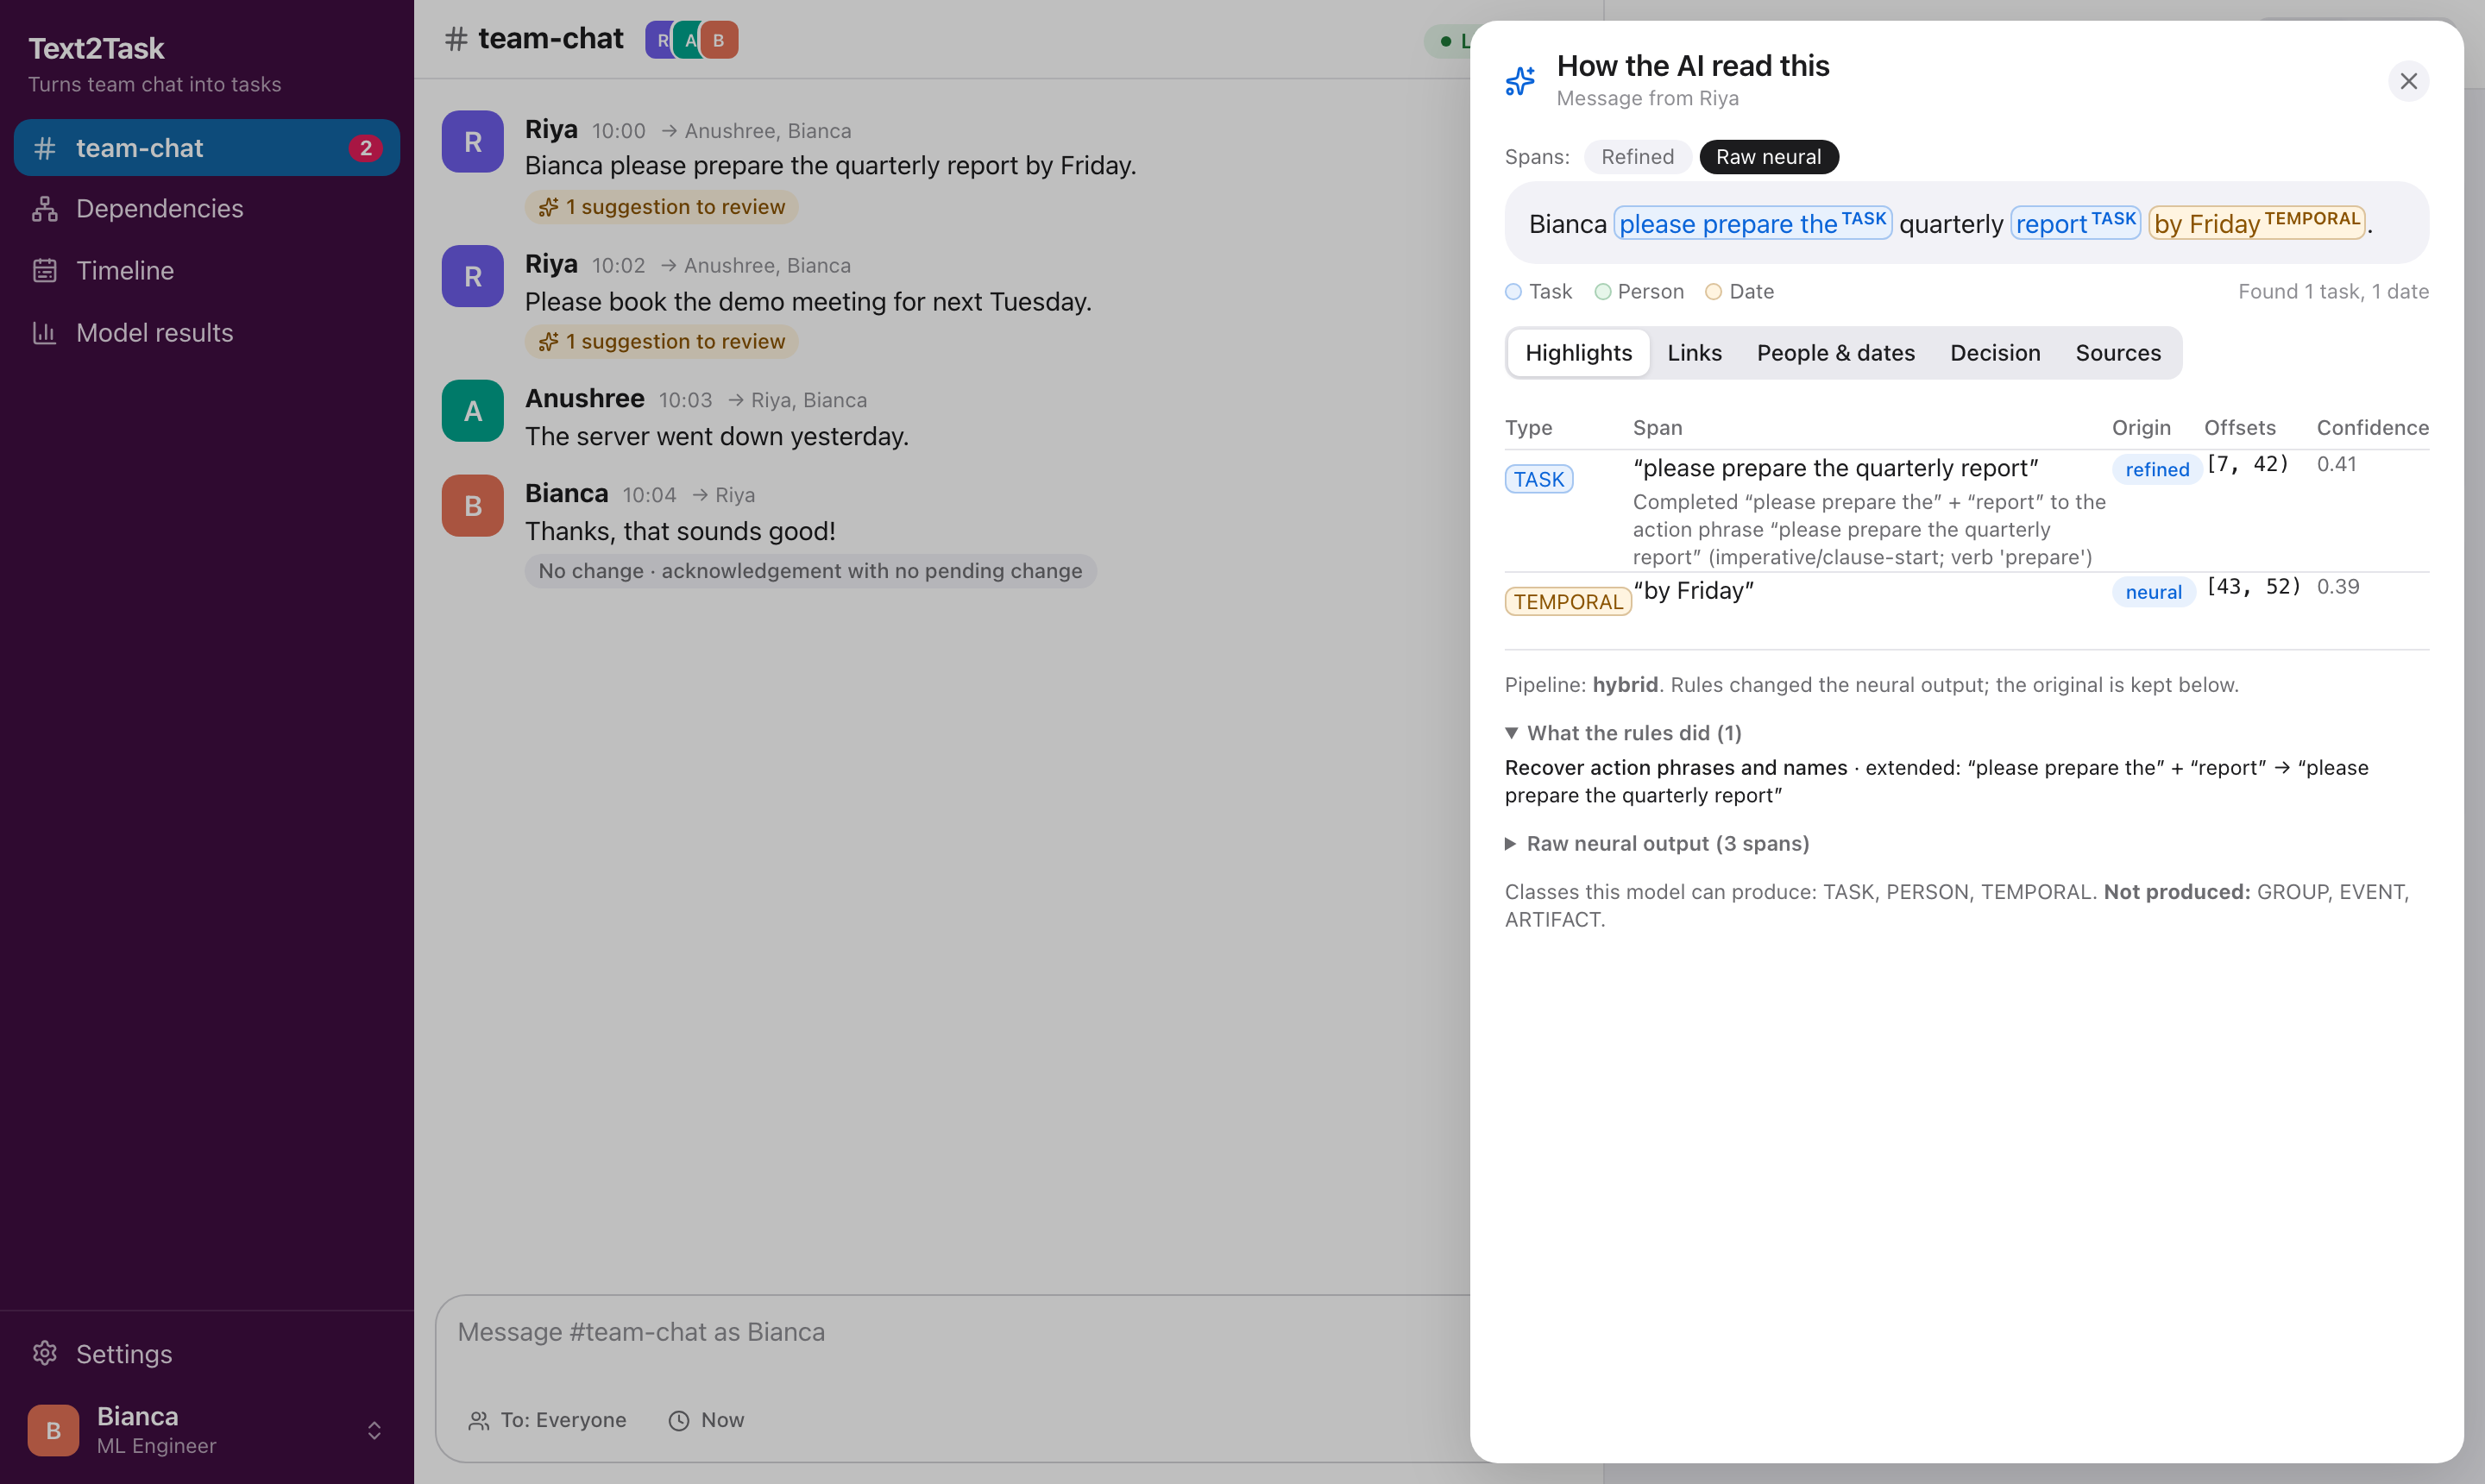
\includegraphics[width=\linewidth, trim=1690 520 20 0, clip]{figures/screenshots/08_inspector_raw_neural.png}
\caption{Raw neural spans}\end{subfigure}
\caption{The inspector for the worked example: two raw TASK fragments joined into one refined span, with the rule recorded.}
\label{fig:shotinspector}
\end{figure}

\begin{figure}[htbp]
\centering
\shot{03_dependency_graph}
\caption{Dependency explorer after the 17-message demo story: a chain, a fan-in, a fan-out, a held cycle-forming edge (red dotted) and a task needing review after its prerequisite was cancelled.}
\label{fig:shotgraph}
\end{figure}

\begin{figure}[htbp]
\centering
\shot{02_date_change_confirmation}
\caption{A task modification proposal: Bianca's requested move to Friday is shown as pending on the task (``New date Fri 13 Nov awaiting OK''); Riya's reply ``Friday is fine.'' became a confirmation that only she may accept.}
\label{fig:shotdate}
\end{figure}

\begin{figure}[htbp]
\centering
\shot{05_ambiguous_referent}
\caption{Ambiguous reference: ``I can review the slides'' matches two open tasks, so the dialog lists both with their match scores and changes nothing until a person chooses.}
\label{fig:shotamb}
\end{figure}

\begin{figure}[htbp]
\centering
\begin{subfigure}[t]{0.49\linewidth}\centering
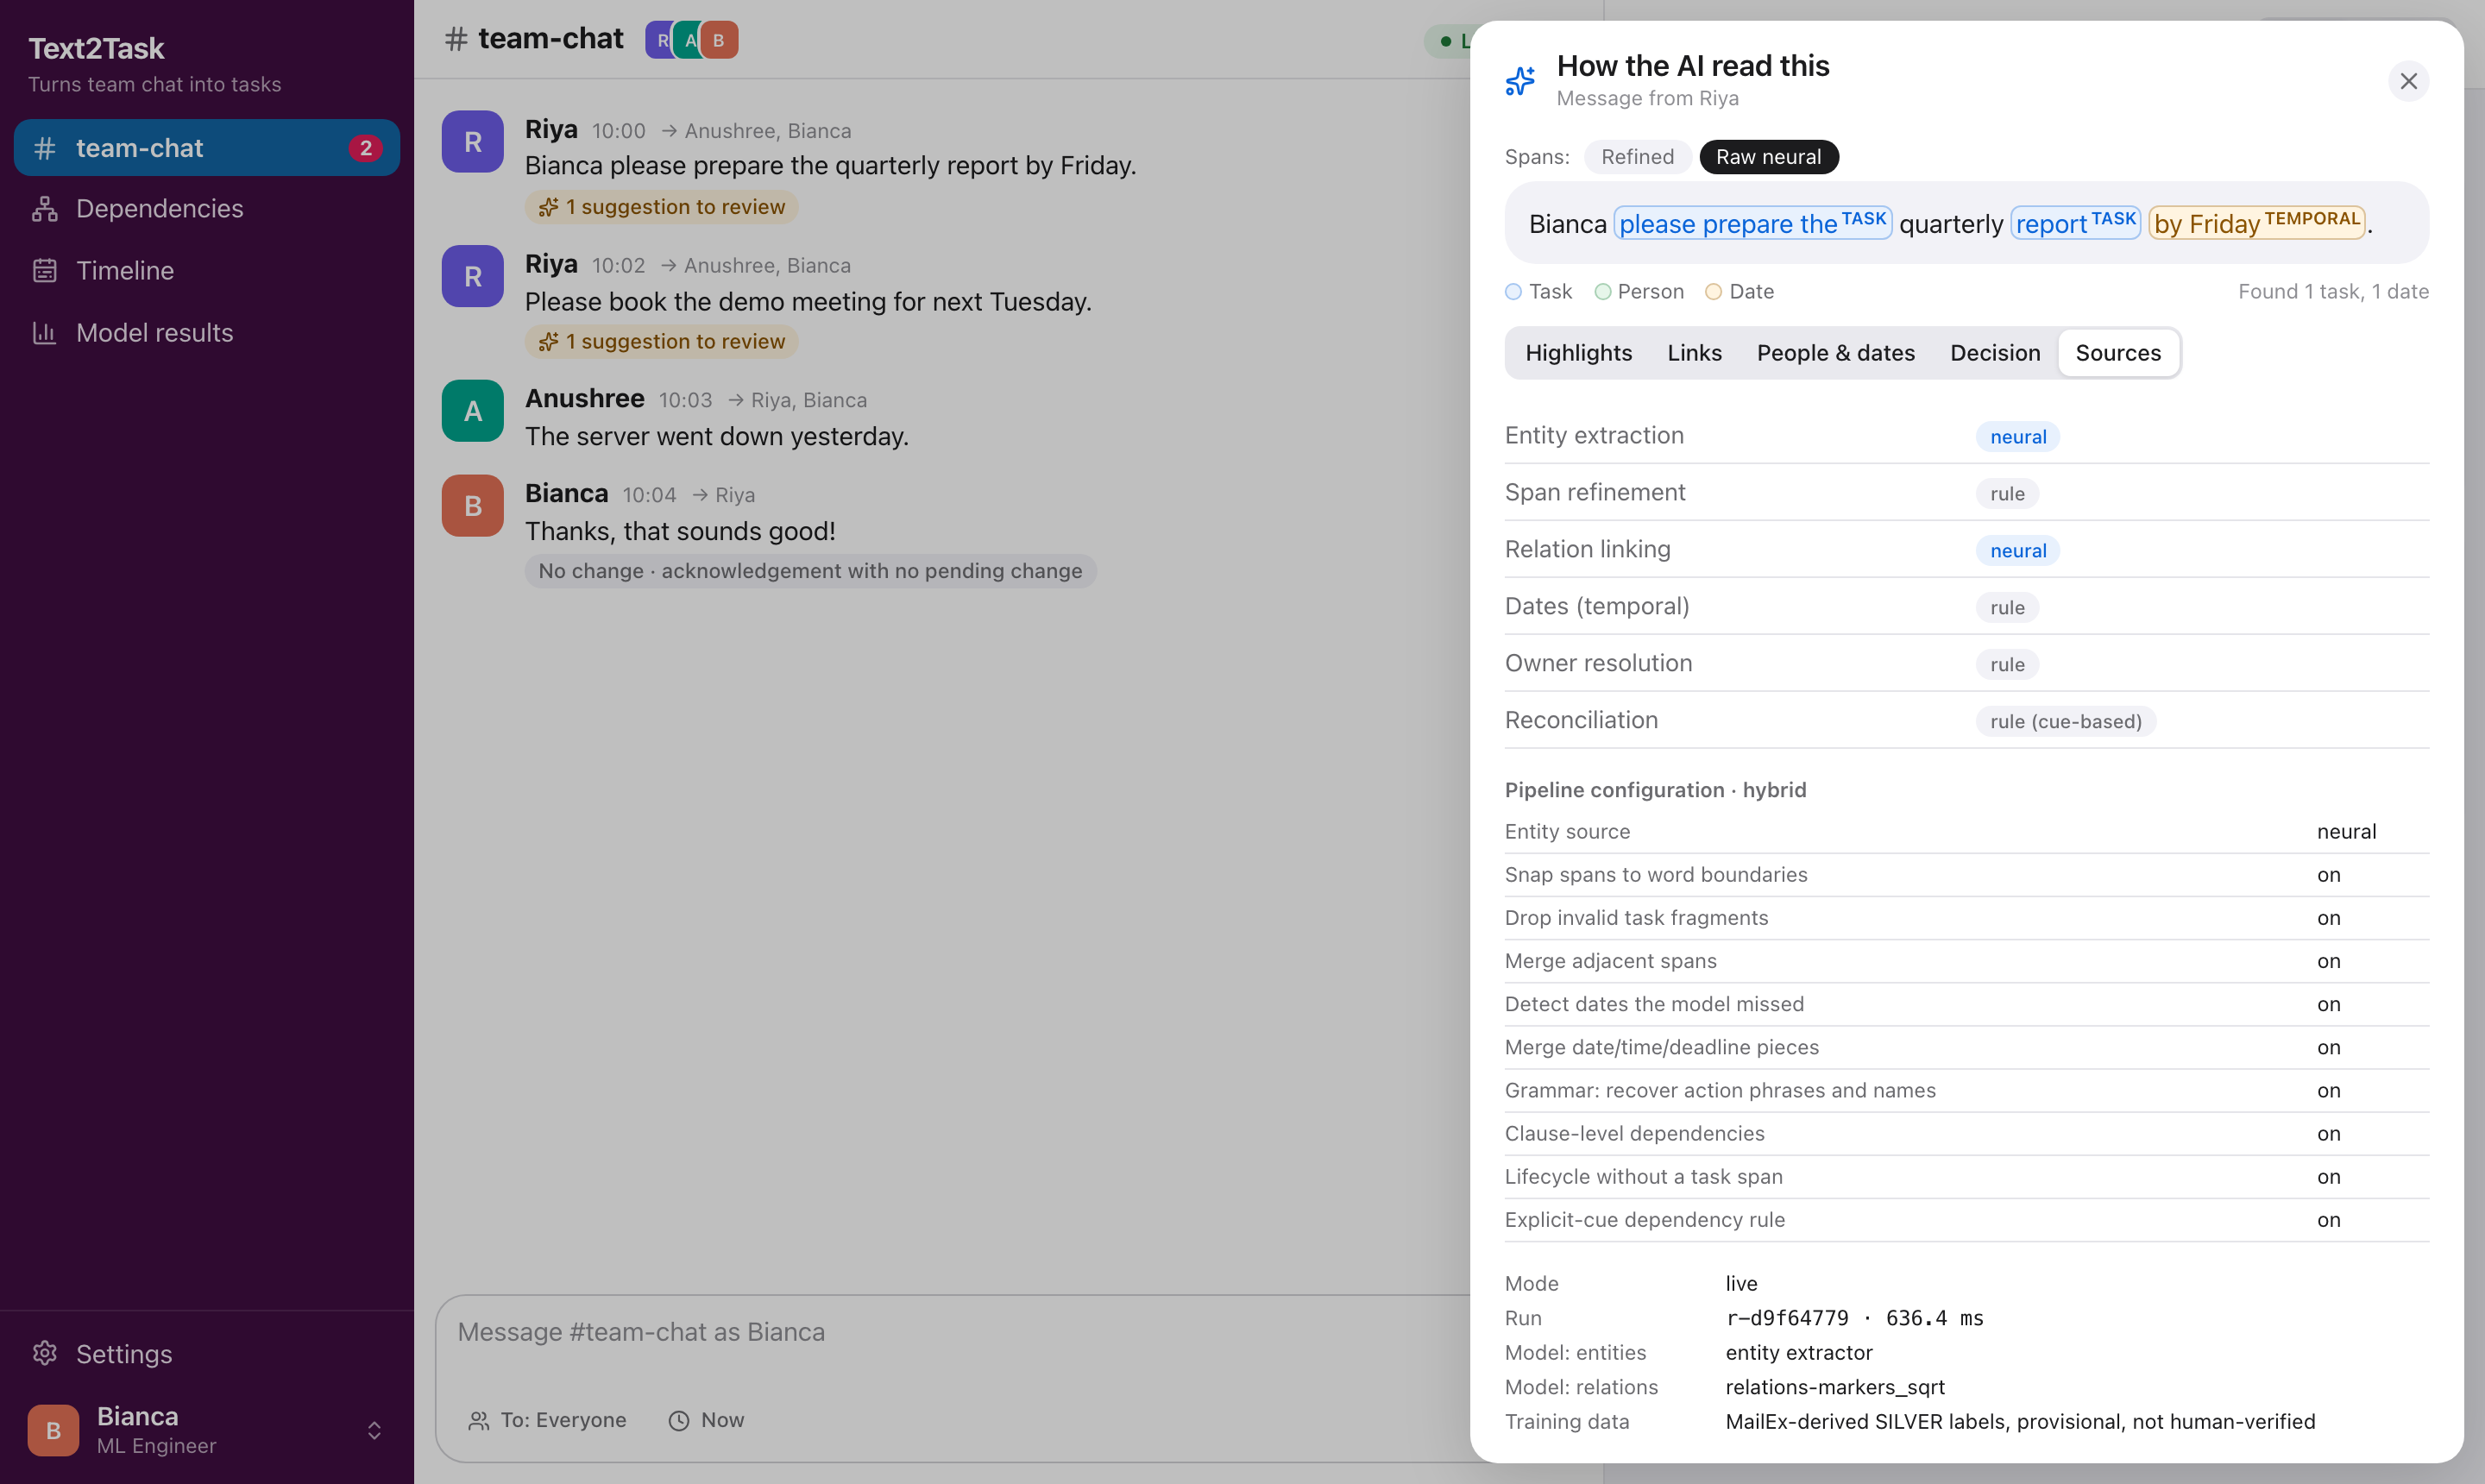
\includegraphics[width=\linewidth, trim=1690 0 20 0, clip]{figures/screenshots/09_inspector_sources.png}
\caption{Sources of every stage and pipeline switches}\end{subfigure}\hfill
\begin{subfigure}[t]{0.49\linewidth}\centering
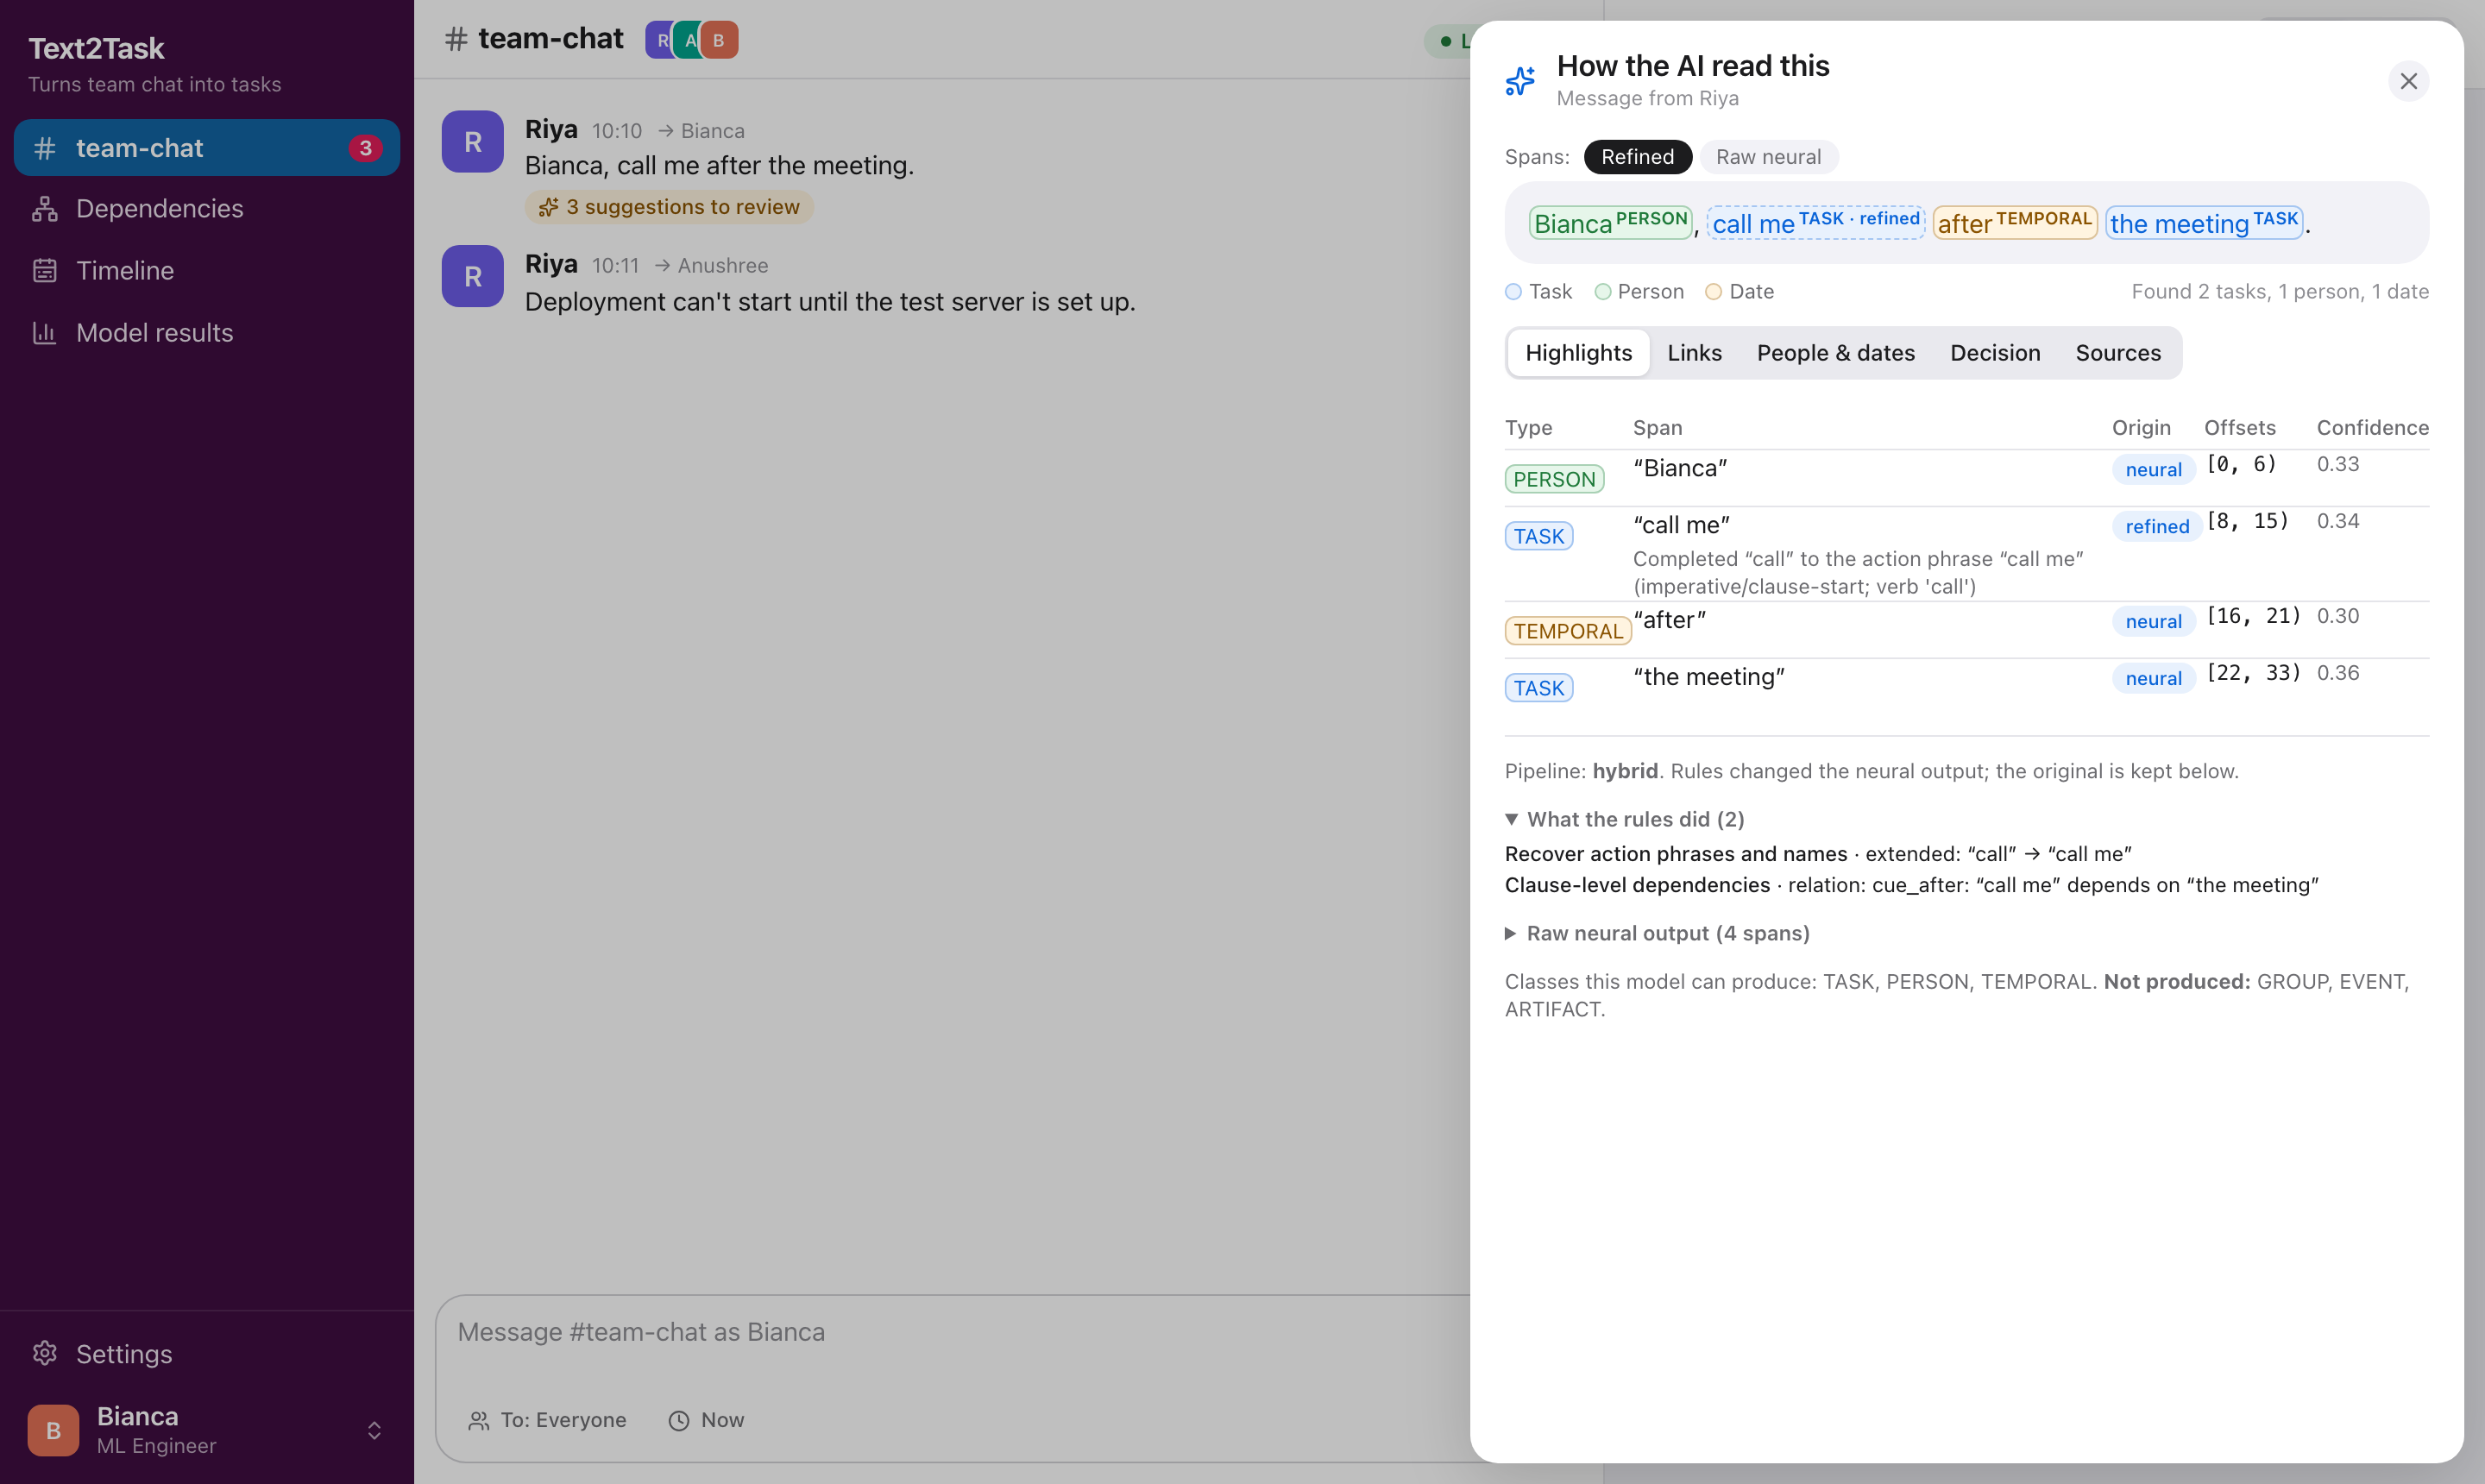
\includegraphics[width=\linewidth, trim=1690 0 20 0, clip]{figures/screenshots/10_failure_case.png}
\caption{Failure: ``call me after the meeting''}\end{subfigure}
\caption{(a) The inspector names the component behind each output and states that labels are not human-verified. (b) A known false positive: \emph{the meeting} is read as a task and \emph{after} as a dependency cue.}
\label{fig:shotfail}
\end{figure}

\begin{figure}[htbp]
\centering
\shot{04_timeline}
\caption{Timeline: open tasks by person on their confirmed due (flag) or planned date; undated tasks are listed, never placed on a guessed day.}
\label{fig:shottimeline}
\end{figure}

\lstinputlisting[style=terminal, caption={Server log excerpt from the screenshot session (verbatim, ports removed).}, label={lst:log}]{figures/screenshots/terminal_server_log.txt}

The system is covered by 362 backend tests, 97 frontend tests with accessibility checks and 20 browser end-to-end tests, 7 of them against the real models.
